\documentclass[a4paper,12pt]{article}
\usepackage{fullpage}
\usepackage{graphicx}
\usepackage{caption}
\usepackage{float}
\usepackage{hyperref}

\hypersetup{
    colorlinks,
    citecolor=blue,
    filecolor=black,
    linkcolor=blue,
    urlcolor=blue
}
\begin{document}
%\selectlanguage{english}
\pagenumbering{Roman}



\title{\begin{Huge}
\textbf{Use Case: Simulation Program for Smart Fridge and Sudoku Solver}
\end{Huge}}
\author{\begin{Large}
Sreenivas, Jonas and Mariusz
\end{Large}}
\date{\today}
\maketitle
\thispagestyle{empty}

\newpage

\pagenumbering{arabic}
\section{Purpose}
This document provides the use case with an UML diagram describing the use case.

\section{Use Case}
The use case for the simulation software is given in a set of points as given below:

\begin{itemize}
\item User starts Simulation Software.

\item User chooses operation mode (Sudoku vs SmartFridge).
\begin{itemize}
\item Based on the choice, users can also make appropriate parameter choices if he is part of User Level 1. User Level 1 includes developers from Sudoku and SmartFridge team who can tune the parameters for the simulation. For other users this choice of parameters is not available.
\end{itemize}
\item Based on the choice from the previous step, the simulation program generates a set of images based on the parameter choices if mentioned or else with default parameter choices based on the inputs from the internal developers of the simulation program.
\item Users can decide to select or reject the images and close the software.
\item The internal code is accessible only to the developers of the simulation program.
\end{itemize}
 \begin{figure}[H]
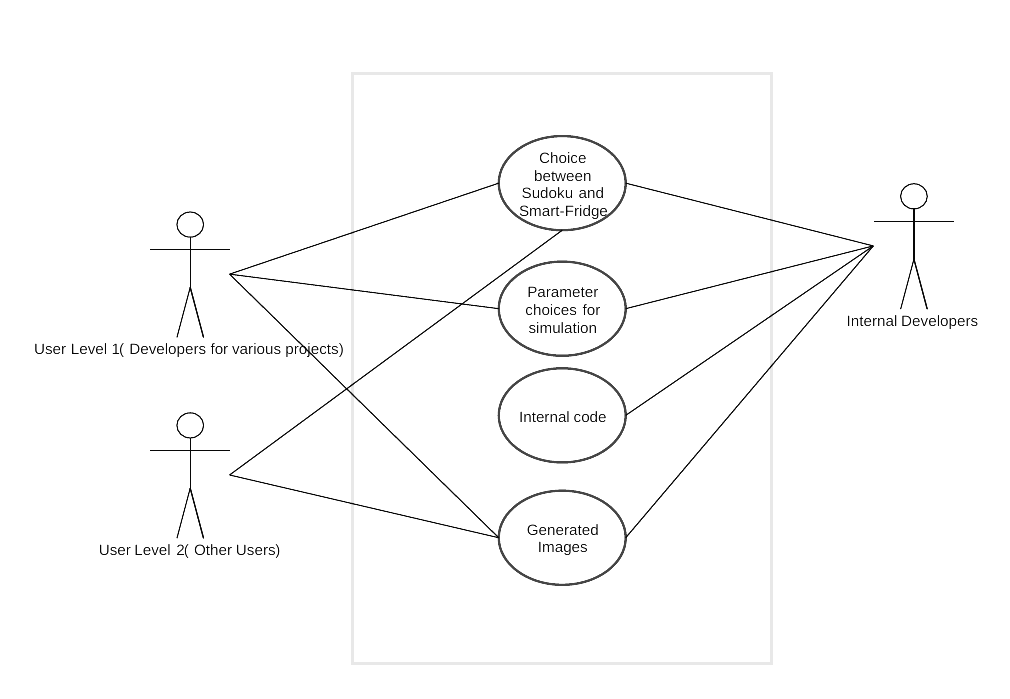
\includegraphics[scale=0.45]{usecase.png}
\caption{Use Case UML diagram}
\end{figure}
\end{document}
